\documentclass{beamer}

\usetheme{boxes}  

\usepackage[applemac]{inputenc}
\usepackage{amsmath}
\usepackage{amssymb}
\usepackage{multicol}
\usepackage{enumerate}

\newcommand{\bfv}{{\bf v}}

%\usebackgroundtemplate{
%\includegraphics[width=\paperwidth,
%height=\paperheight,brightness=0.1]{images/newtest1.jpg}
%}

\title{A Quick Guide to Organizing Computational Biology Projects}
\author{William Stafford Noble}
\date{PLoS Computational Biology 2009}

\setbeamercovered{invisible}
\setbeamertemplate{navigation symbols}{}

\begin{document}

\begin{frame}
\titlepage
\end{frame}

%\usebackgroundtemplate{
%\includegraphics[width=\paperwidth,
%height=\paperheight,brightness=0.1]{images/newtest1.jpg}
%}

\begin{frame}{Motivation}
You are at the start of a new project and want to 

\begin{itemize}
\item pre-process data

\item run data through several models, algorithms (code still to be written by you)

\item write regular progress reports
\end{itemize}

Excel, csv, .R, preliminary results, plots, final results, reports.

\bigskip

{\color{blue} All files in one folder may not be the best approach.}

\pause

\begin{block}{}
{\color{red}$\leadsto$} Author describes {\color{blue} ``one good strategy''} (personal experience) for carrying out computational experiments
\begin{itemize}
\item organizing files and directories, and documenting progress.
\end{itemize}
\end{block}
\end{frame}


\begin{frame}{Core guiding principles}
Someone unfamiliar with your project should be able to look at your computer files and understand in detail what you did and why.

\pause

\medskip

{\color{red}�Someone?}

\pause

\begin{itemize}
\item someone who read your published article and wants to try to reproduce your work,

\item a collaborator,

\item a future student working in your lab,

\item your research advisor,

\item most commonly, however, {\color{blue} that �someone� is you}.
\end{itemize}
\end{frame}


\begin{frame}{Second principle}
Everything you do you will {\color{blue} probably have to do over again}.

\begin{itemize}
\item flaws in algorithm,

\item new data,

\item broader parametrization,

\item reviewers wants modifications.
\end{itemize}
\end{frame}


\begin{frame}{File and directory organization}
Common root directory, keep it {\color{blue} chronological}.

\begin{center}
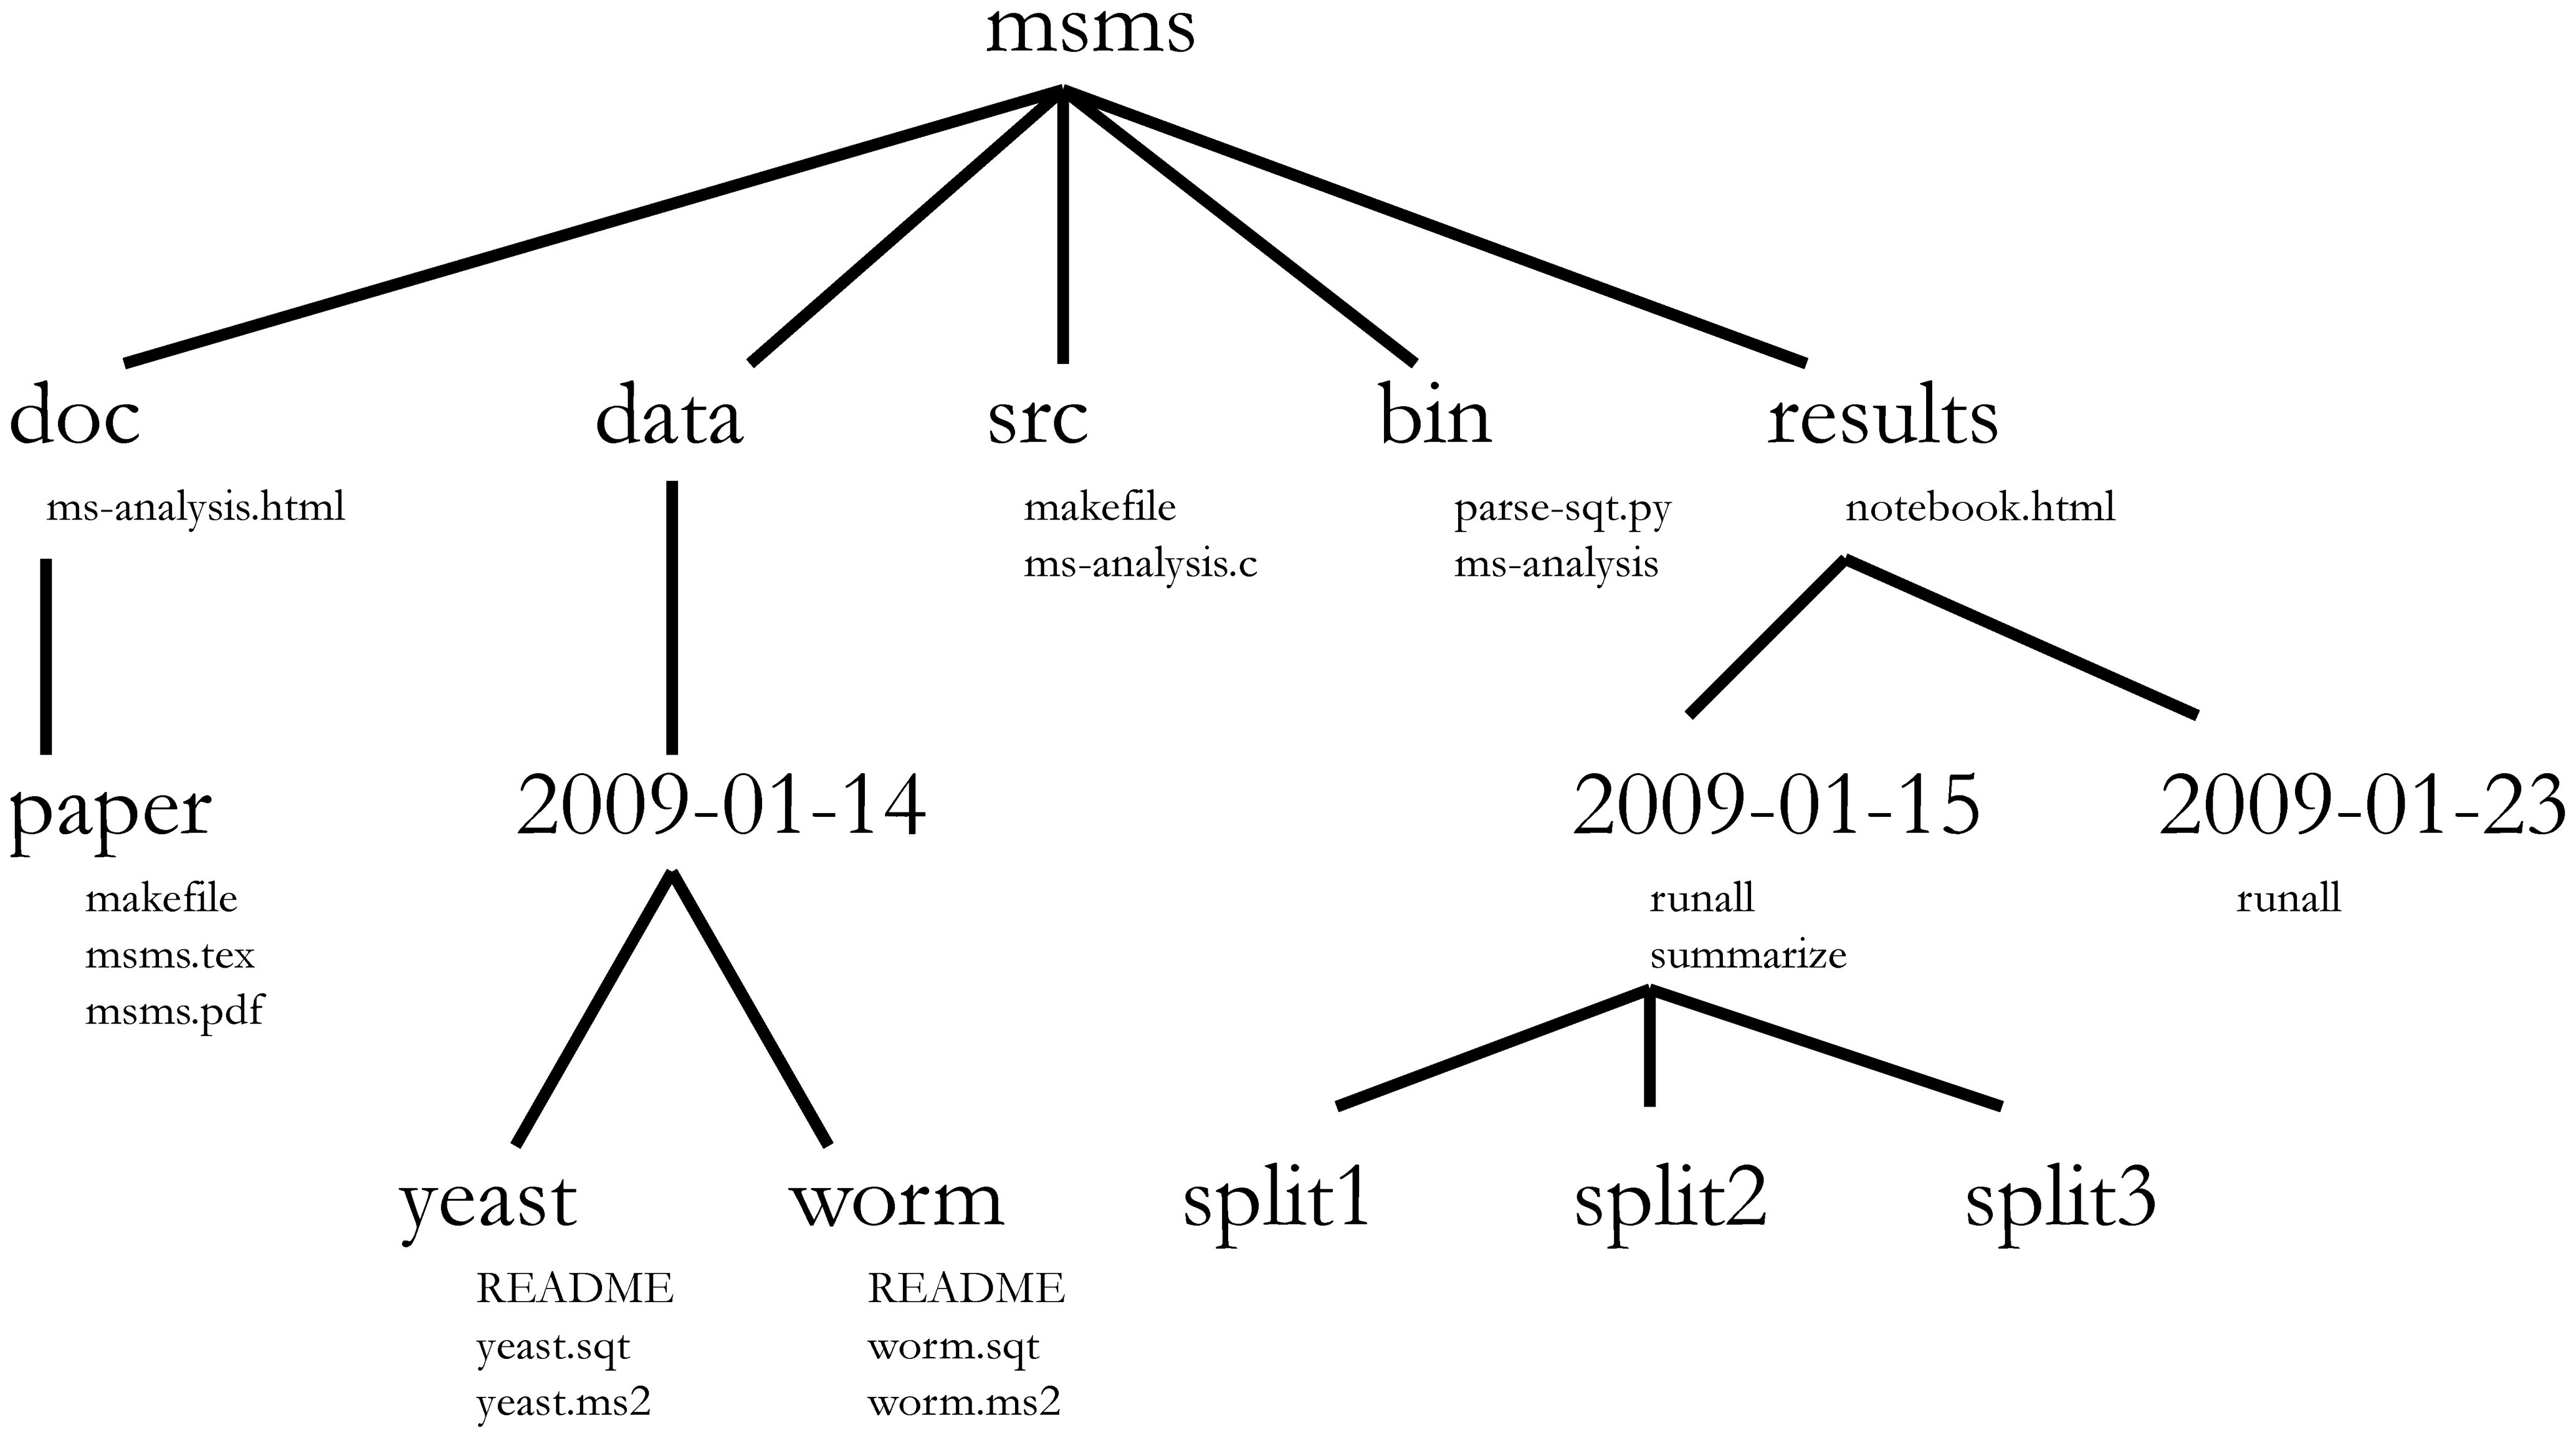
\includegraphics[width=.95\textwidth]{tree.jpg}
\end{center}
\end{frame}


\begin{frame}{Lab notebook}
Keep in {\it results} directory

\begin{itemize}
\item record observation, your interpretation and conclusion, questions, future ideas.

\item esp.\ when experiment fails or doesn't give expected result. {\color{blue} {\color{red} why} this is a fail may not be obvious to {\it that someone}.}

\item add notes from conversations, emails, meetings with advisor.

\item If you want, put notebook online for project team to read.
\end{itemize}
\end{frame}


\begin{frame}{Single experiment}

{\color{blue} readme} file for each

\begin{itemize}
\item have a file {\color{blue} runall} to make everything automatic, best if this also {\color{blue}�creates summary}. {\it e.g.\ run R script first, save plots, put them in \LaTeX{} or Word document.}

\item avoid editing intermediate files by hand

\item use relative pathnames, not absolute

\item if script has long run time use things like

{\ttfamily if (output does not exists) perform operation; otherwise next step}

\item or use function {\color{blue} summarize} that is called in last line of runall. summarize should then also work with {\color{blue} partial results}.

\item outputs should be {\color{blue} temporary files} to avoid taking partial results for final/full results.
\end{itemize}
\end{frame}

\end{document}